\chapter{Design and Implementation}\label{C:di}

\section{Design}
This section will cover the design within the context of the overall application of Whiley-to-WebAssembly. Aswell as how implementation and design challenges around the compiler step being implemented.

\subsection{Architecture Overview}

To look at the architecture we have to take the whole Whiley compiler into account. Compilers are normally built around a pipeline architecture, this is the same for Whiley. The source code will get processed by the first step in the compiler and then passed on to the next as seen in figure \ref{fig:arc}. 

\begin{figure}[H]
  \centering
  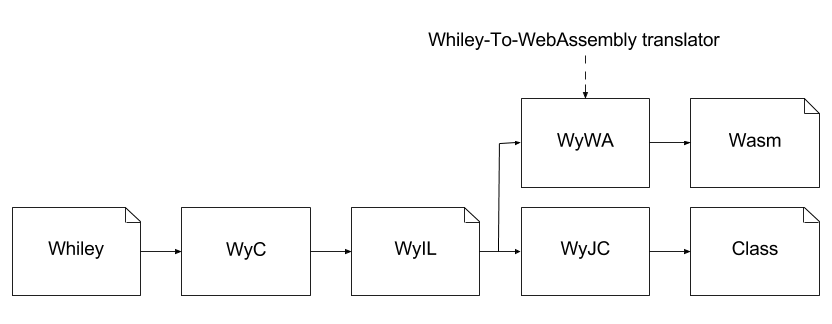
\includegraphics[width=0.8\textwidth]{My_Preposed_Extention}
  \caption{Whiley Compiler Pipeline}
  \label{fig:arc}
\end{figure}

Then a WyIL file is passed to Whiley-to-WebAssembly translator. The translator will construct and output a wasm file. 


\subsection{Design Challenges}\label{subsec:didc}

Throughout this project there have been several important challenges that needed to be overcome. These challenges will be discussed within this section as well as how they were over come. 

\paragraph{}
Conversion of unstructured control flow used by the WyIL files (seen in figure \ref{fig:wyil}) to the structured control flow of Web Assembly and branching, as mentioned in \ref{subsec:wad}, is a challange. The technique that is used is based on how Enscripton transforms LLVM to JavaScript \cite{Zakai:2011:ELC:2048147.2048224}.
%To add more.

\paragraph{}
Also a challenge is the heap and pointers in wasm are addressable memory (the heap) and integers that represent locations in that memory (pointers). The design takes values intended for the heap and assigns them a location. The location is then used to reference them again. 
%Need more consistent nameing sceam.

\paragraph{}
Arrays and records in Whiley, as mentioned in section \ref{subsec:wy} both have value semantics.% Add more detail about what i mean by value semantics.
 The challenge is to ensure that these semantics are not changed when compiled from Whiley to wasm. To ensure this, every time a reference is assigned or used in a method a copy is created. 


\paragraph{}
Finally type information at runtime is important for casting and managing referenced types on the heap. To manage this type information from the WyIL file needs to be stored in wasm. %Add more explination here.


\section{Implementation}

This section covers the implementation of the abstract syntax tree along with the implementation of the design challenges from \ref{subsec:didc}.

\subsection{Abstract Syntax Tree}

The abstract syntax tree (AST) is made to represent wasm as specified in \cite{11_webassembly/spec_2016} and \cite{10_gohman_bastien_wagner_2016}.  This is added to improve the representation of wasm in code. Previously wasm was represented as a string, this creates problems when it comes to code modification. As a result the programs representation became tied in with creation.

\begin{figure}[H]
  \centering
  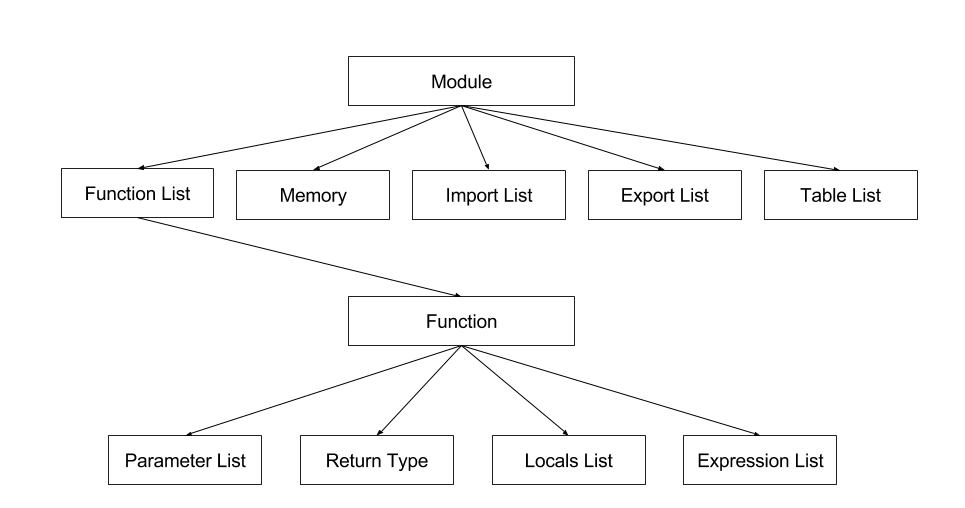
\includegraphics[width=0.8\textwidth]{AST}
  \caption{Simplified Web Assembly AST}
  \label{fig:ast}
\end{figure}

\paragraph{}
Figure \ref{fig:ast}, shows the overall structure of the AST when constructed. Modules the overall structure of the file storing important information like the size of the heap (Memory) and the list of functions defined (Function List). Functions have information about the parameters, locals, return type and expressions that are evaluated within the function. The diagram is missing the large amount of expressions that have been implemented. 

\subsection{Design Challenge Solutions}\label{subsec:didcs}

\paragraph{Unstructured Control Flow}
is transformed into structured control flow using a loop that can loop arbitrarily many times around a large collection of if statements. This transformation can be seen in figure \ref{fig:wtw}. If there are no labels in the WyIL code then Transform 1 will happen regardless. Each transform wraps code within a if statements that checks against the pc value. The pc value is set so that the first statement is always executed. 

\begin{figure}[H]
  \centering
  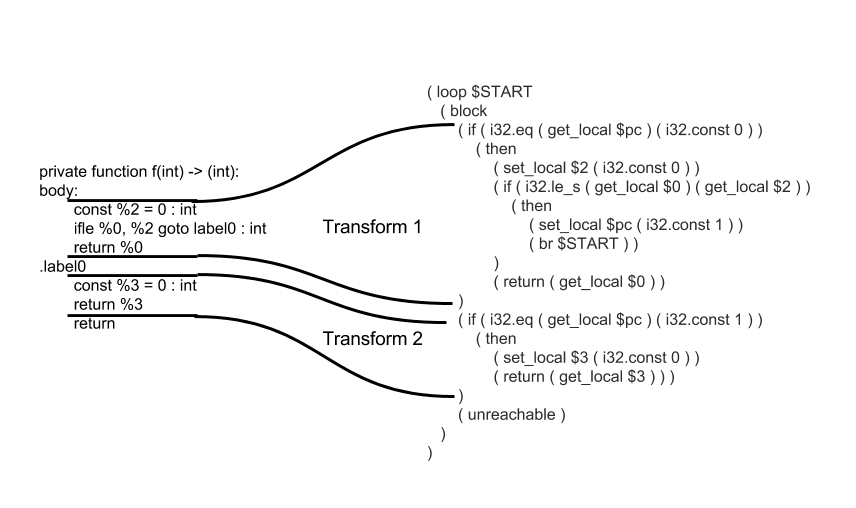
\includegraphics[width=0.8\textwidth]{StatementTransform}
  \caption{WyIL to Web Assembly Transform}
  \label{fig:wtw}
\end{figure}

\paragraph{The Heap and Pointers}
are represented by integers in wasm. This can be seen in figure \ref{fig:hlo}, where the first location on the heap is a pointer to the end and free space. When a new value is added to the heap the base address updates to the new end of heap. This implementation uses a bump pointer and is not efficient because, when memory is no longer needed it cannot be used again. Values that are created and then stored on the heap will keep a reference to the start of that value.

\begin{figure}[H]
  \centering
  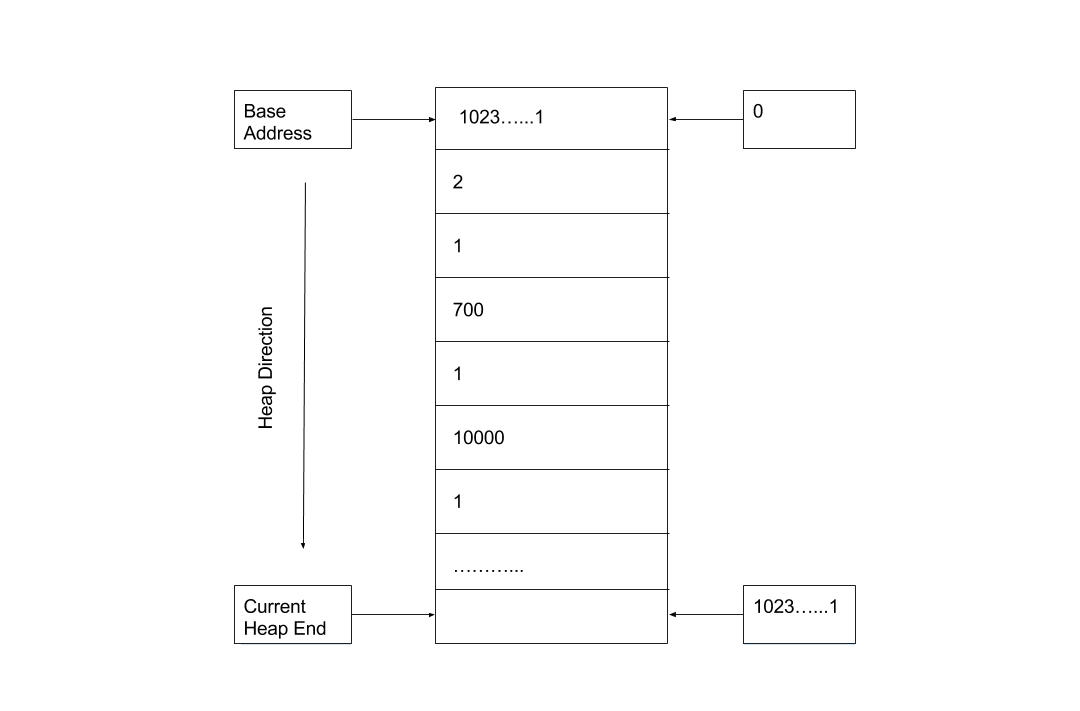
\includegraphics[width=0.8\textwidth]{HeapLayout}
  \caption{Heap Layout}
  \label{fig:hlo}
\end{figure}

%% TODO: Fix this so it is split into two differnet paragraphs.
\paragraph{Arrays and records}
 are stored on the heap in the same structure, see figure \ref{fig:arl}, this allows runtime copying function to be applied to the heap without large amounts of work. This implementation does use more space on the heap but it simplifies memory management.
 
\begin{figure}[H]
  \centering
  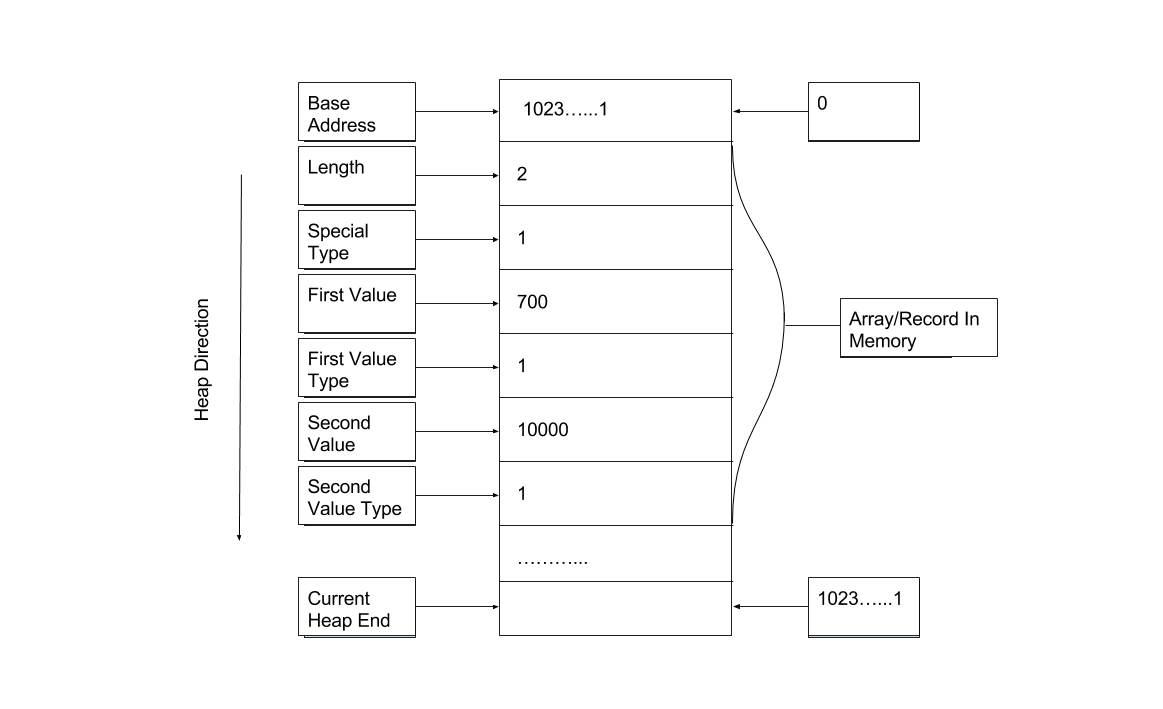
\includegraphics[width=0.8\textwidth]{ArrayLayout}
  \caption{Array and Record Layout on the Heap}
  \label{fig:arl}
\end{figure}

%Cover some information about the runtime copy function.

\paragraph{Type Information}
is stored for each variable and reference as well as values in data structures on the heap as seen in figure \ref{fig:arl}. Each type is mapped to an integer at compile time. This implementation is considered to as a closed world assumption. This means no types from outside the program can be used at runtime this is efficient but limiting. This is efficient because extensive type checking does not need to be made but it does restrict types available to define in the program. Arrays and record type information differs from non referenced values by having their type information in more than one place. The type stored with the reference tells whether it is a array, or a record, nothing else. The structure on the heap seen in figure \ref{fig:arl}, has extra information stored after the length value. For arrays this represents the super-type/type of elements within the array and for records this represents the types and names of fields. 
